\chapter{Introduction\label{cha:chapter1}}

% i sent you my comments by email. in general, i would recommend to restructure your introduction (and thesis) as follows:
% 1. your goal is to approximate a wide class of hysteretic processes by neural networks.
% 2. hysteretic processes have memory, introduce different hysteresis operators, say that Preisach is quite general, and it can be approximated by a linear combination of generalized (nonlinear) plays.
% 3. RNNs can approximate processes with memory, but standard architectures such as LSTM are not good enough.
% 4. that's why you develop a new architecture, namely HNN - this is your first result! it is a realization of a linear combination of nonlinear plays and hence approximates any Preisach operator (cf. item 2)
% 5. you compare hnn with lstm for learning hysteretic input-output relations and show that hnn is better. this is your second result!
% 6. you generalize a hysteretic market model from Dima and Kreiji by including N-agents. this is your third result!
% 7. you learn this model using hnn and lstm and show that hnn is better. this is your fourth result!

% ...n the introduction part, you should focus on hysteretic NN
% not on the stock market
% the stock market is just one of the applications

% hysteresis behaviours in trading strategies cite from dima. cite from other financial papers.
% inside dima's paper, he only use D agents to simulate 
% we use N agents and D agents (results)
% in order to trade, trading we need to use hysteresis network.
% lstm to predict stock, don't take account into hysteresis behaviours and it fails(?)
% (why we need to use hysteresis in financial market, from other paper)
% even to predict hysteresis process
% implement neural network with these specific architecture
% use hnn, train efficiently. (results)
% (new results), train stock market results  is even difficult.
% and analysis the results. 
% add plots, can predict price distributions. 
% organization.

%%%%%%%%%%%%%%%%%%%%%%%%%%%%%%%%%%%%%%%%%%%%%%%%%%%%%%%%%%%%%%%%%%%%%%%%%%%%%%%%%%%%%%%%%%%
% 1. Your goal is to approximate a wide class of hysteretic processes by neural networks.
\textit{Hysteresis} (see \myfigref{fig:chapter1:hysteresis-loop,fig:chapter1:non-ideal-relay,fig:chapter1:stop,fig:chapter1:play}) is defined as a \textit{rate independent} process with \textit{memory effect} \citep{visintin2013differential}. It's ubiquitous in various fields, including microelectronics \lackref{}, thermodynamics \lackref{}, materials \lackref{}, mechanics \lackref{}. economics \citep{belke2013exchange,gocke2002various,belke2014hysteresis}, etc. The nonlinear operators like \textit{non-ideal relay operator} (see \myfigref{fig:chapter1:non-ideal-relay}), \textit{stop operator} \citep{krejci1996hysteresis} (see \myfigref{fig:chapter1:stop}), \textit{play operator} \citep{krejci1996hysteresis} (see \myfigref{fig:chapter1:play}) and their generalizations are used as essential blocks to model dynamical systems with hysteresis.
\todo{show this statement is correct} Preisach-type model, constructed as a superposition of non-ideal relays, is quite general in applications \lackref{} and it's equivalent to a linear combination of \textit{generalized plays}, namely, a \textit{generalized Prandtl-Ishlinskii operator of play-type} \citep{visintin2013differential}. % page 111, is it true?

In this thesis, we want to approximate a wide class of hysteretic processes, Preisach-type model, by neural network. Intuitively, recurrent neural network (RNN) \lackref{} is a optional approach to approximate systems with \textit{memory} \todo{explain what's memory here} since it allow previous output to be used as input while having hidden states. \citet{wang2018prandtl} applied Internal Time-Delay RNN to describe the hysteresis and showed promising performance that their network  described both the major and minor hysteresis loops well. However, they preprocessed input by the ground-truth play operator and tried to find relationship between output and processed input. In other words, they didn't approximate \textit{nonsmooth} operator, like play operator, in their model. We also checked Long Short Term Memory (LSTM) networks \citep{hochreiter1997long}, the state-of-the-art architecture of RNN, and found that it didn't perform well enough to reveal the relationships between outputs and original input in hysteretic systems. % \citet{wei2000constructing} proposed a propulsive neural unit (PNU) to assist hysteresis simulation. 
In order to achieve better performance, \textbf{we develop a new neural network architecture, namely hysteretic neural network (\text{HNN}) (see \myfigref{fig:chapter1:nn-arch})}. It is a realization of a linear combination of generalized plays and hence it's able to approximate any \todo{add theorem} \textit{Preisach operator} \citep{visintin2013differential}. Restated, herein we approximate Preisach-type model via learning unknown generalized Prandtl-Ishlinskii operator.

% second results
Given an observation $(x_n, y_n) \, (n=1,\ldots, N)$ underlying hysteretic input-output relations, both LSTM and HNN minimize mean square error (MSE) between predicted target $\hat{y}_n$ and observed target $y_n$. \textbf{It shows HNN outperforms LSTM by comparing root mean square error (RMSE). In particular, HNN is able to reconstruct \textit{minor hysteresis loops} well whereas LSTM fails.} \todo{should I put some plots here to show that hnn outperforms lstm}
% \mytodo{5. you compare hnn with lstm for learning hysteretic input-output relations and show that hnn is better. this is your second result!}

% 5. you compare hnn with lstm for learning hysteretic input-output relations and show that hnn is better. this is your second result!

% In this thesis, we provide a new architecture network to approximate a wide class of hysteretic processes with \textit{local memory} \lackref{local memory can be called markovian hysteresis nonlinearities}.
% 2. hysteretic processes have memory, introduce different hysteresis operators, say that Preisach is quite general, and it can be approximated by a linear combination of generalized (nonlinear) plays.
%%%%%%%%%%%%%%%%%%%%%%%%%%%%%%%%%%%%%%%%%%%%%%%%%%%%%%%%%%%%%%%%%%%%%%%%%%%%%%%%%%%%%%%%%%%


%%%%%%%%%%%%%%%%%%%%%%%%%%%%%%%%%%%%%%%%%%%%%%%%%%%%%%%%%%%%%%%%%%%%%%%%%%%%%%%%%%%%%%%%%%%
% 2. hysteretic processes have memory, introduce different hysteresis operators, say that Preisach is quite general, and it can be approximated by a linear combination of generalized (nonlinear) plays.
%%%%%%%%%%%%%%%%%%%%%%%%%%%%%%%%%%%%%%%%%%%%%%%%%%%%%%%%%%%%%%%%%%%%%%%%%%%%%%%%%%%%%%%%%%%

% \textit{Hysteresis} (see \myfigref{fig:chapter1:hysteresis-loop,fig:chapter1:non-ideal-relay,fig:chapter1:stop,fig:chapter1:play}) is defined as a \textit{rate independent} process with \textit{local memory}  \citep{visintin2013differential}. The \textit{nonsmooth} operators like \textit{stop operator} \citep{krejci1996hysteresis} (see \myfigref{fig:chapter1:stop}), \textit{play operator} \citep{krejci1996hysteresis} (see \myfigref{fig:chapter1:play}), \textit{Preisach operator} \citep{visintin2013differential} and their generalizations are used as essential blocks to model dynamical systems with hysteresis. Hysteresis effects are encountered in many different fields of science, such as magnetic hysteresis, ferroelectric hysteresis, mechanical hysteresis, superconducting hysteresis, adsorption hysteresis\lackref{}, etc. More recently, applications of these nonlinearities range from medicine \citep{castellano2010thresholds,gleeson2011high,parshani2010epidemic} and biology \citep{friedman2014hysteresis} to economics and finance \lackref{}.
% Especially in economics and finance fields, Preisach-type models, using \textit{non-ideal relay operator} (see \myfigref{fig:chapter1:non-ideal-relay}), have been used as tool to describe the macro dynamics of economic systems, which deliver hysteresis at both micro and macro levels as such a procedure of aggregation over individual heterogeneous agents.
% Hysteresis in economics, typically based on suck adjustment costs\lackref{}, has been also well investigated in the relationship between economic facts and unemployment rate, exports and exchange rate  \citep{belke2013exchange,gocke2002various,belke2014hysteresis}. Naturally, an attempt to obtain quantitative models of these empirical observations motivated the use of the play operator and more complex models of hysteresis in the financial market trading context. 
% \lackref{Amable et al. (1994) who applied a model of hysteresis to the study of foreign trade, Lang and Peretti (2009) also found hysteresis in the dynamics of the unemployment rate, and Belke and Göcke (2001) documented hysteresis in the relationship between aggregate employment and the exchange rate.}.

% \mytodo{add hysteretical background, what's hysteresis, why hysteresis?}
\begin{figure}[htb!]
    \centering
    \subfloat[hysteresis loops]{
        \scalebox{0.77} {
        \documentclass{article}
\usepackage{tikz}
\begin{document}
  \begin{tikzpicture}
    \draw[] (-3,-3) .. controls (2.5,-3) and (-0.5,3) .. (3,3)
             .. controls (-2.5,3) and (0.5,-3) ..(-3,-3);
    \draw[-latex] (-4,0) -- (4,0)node[below]{$u$};
    \draw[-latex] (0,-4) -- (0,4)node[left]{$x$};
    % \draw[dashed] (-4,-3) -- (4,-3);
    % \draw[dashed] (-4,3) -- (4,3);
    
    \draw[dashed] (-3,0)node[above]{$u_1$} -- (-3,-3)node[below]{$A$};
    \node[right] at (0.7, 0) {$B$};
    \draw[dashed] (3,0)node[above]{$u_2$} -- (3,3)node[above]{$C$};
    \node[left] at (-0.7, 0) {$D$};

\end{tikzpicture}
\end{document}
        }
        \label{fig:chapter1:hysteresis-loop}
    }
    \subfloat[non-ideal relay]{
        \scalebox{1.0} {
        \documentclass{standalone}
\usepackage{pgfplots}
\pgfplotsset{compat=1.11}
\begin{document}
% Place the TikZ picture in a figure environment.
%\begin{figure}[htb]
% h: here, t: top, b: bottom, p: page of float
%% https://tex.stackexchange.com/questions/39017/how-to-influence-the-position-of-float-environments-like-figure-and-table-in-lat
%% ! indicates that some restrictions should be ignored (discussed later)
%% h indicates that the float is allowed to be placed inline
%% t indicates that the float is allowed to go into a top area
%% b indicates that the float is allowed to go into a bottom area
%% p indicates the the float is allowed to go on a float page or column area

    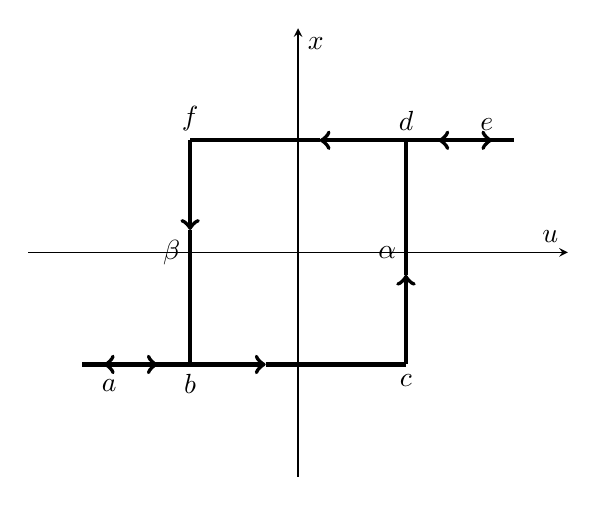
\begin{tikzpicture}
        \begin{axis} [
            xmin=-2.5, xmax=2.5, ymin=-2, ymax=2, 
            % grid=both,
            ylabel={$x$}, xlabel={$u$},
            % xtick={-2,-1.5,...,2}, ytick={-2,-1.5,...,2},
            % xticklabel style={font=\tiny, xshift=0.5ex},
            % yticklabel style={font=\tiny, yshift=0.5ex},
            axis line style={->},
            axis x line=middle,
            axis y line=middle,
            ticks=none
        ]
        \addplot+[line width=1.5pt, color=black, dashed, ->, mark=none, domain=-1.3:-1.8] {-1};
        \addplot+[line width=1.5pt,color=black, solid, ->, mark=none, domain=-2:-1.3] {-1};
        \addplot+[line width=1.5pt,color=black, solid, ->, mark=none, domain=-2:-0.3] {-1};
        \addplot+[line width=1.5pt,color=black, solid, mark=none, domain=-0.3:1] {-1};

        \addplot+[line width=1.5pt,color=black, solid, mark=none, ->,domain=1.3:1.8] {+1};

        \addplot+[line width=1.5pt,color=black, solid, mark=none, ->,domain=2:1.3] {+1};
        \addplot+[line width=1.5pt,color=black, solid, mark=none, ->, domain=1.3:0.2] {+1};
        \addplot+[line width=1.5pt,color=black, solid, mark=none, domain=0.2:-1] {+1};

        \draw[line width=1.5pt,color=black, solid, mark=none, ->] (1, -1) -- (1, -0.2);
        \draw[line width=1.5pt,color=black, solid, mark=none] (1, -0.2) -- (1, +1);

        \draw[line width=1.5pt,color=black, solid, mark=none, ->] (-1, +1) -- (-1, +0.2);
        \draw[line width=1.5pt,color=black, solid, mark=none] (-1, +0.2) -- (-1, -1);

        \node[below] at (-1.75,-1.05) {$a$};
        \node[below] at (-1,-1) {$b$};
        \node[below] at (1,-1) {$c$};
        \node[above] at (1,1) {$d$};
        \node[above] at (1.75,1) {$e$};

        \node[above] at (-1,1) {$f$};
        
        \node[left] at (-1,0) {$\beta$};
        \node[left] at (1,0) {$\alpha$};
        
        \end{axis}
    \end{tikzpicture}

\end{document}
        }
        \label{fig:chapter1:non-ideal-relay}
    }
    \hfill
    \subfloat[stop]{
        \input{./tikz/stop-def}
        \label{fig:chapter1:stop}
    }
    \subfloat[play]{
        \documentclass{standalone}
\usepackage{pgfplots}
\pgfplotsset{compat=1.11}
\begin{document}
% Place the TikZ picture in a figure environment.
%\begin{figure}[htb]
% h: here, t: top, b: bottom, p: page of float
%% https://tex.stackexchange.com/questions/39017/how-to-influence-the-position-of-float-environments-like-figure-and-table-in-lat
%% ! indicates that some restrictions should be ignored (discussed later)
%% h indicates that the float is allowed to be placed inline
%% t indicates that the float is allowed to go into a top area
%% b indicates that the float is allowed to go into a bottom area
%% p indicates the the float is allowed to go on a float page or column area

    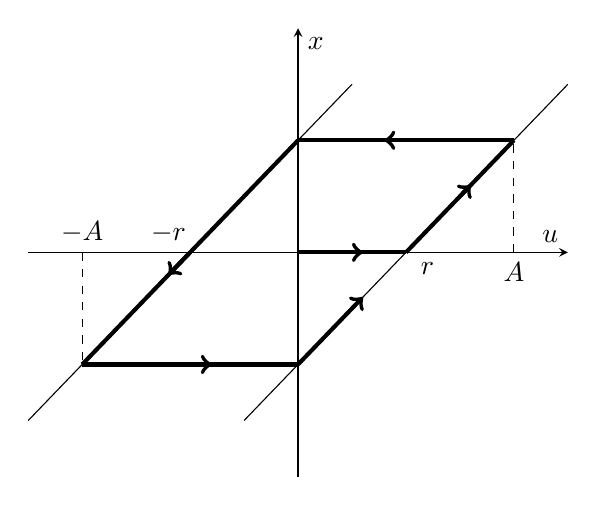
\begin{tikzpicture}
        \begin{axis} [
            xmin=-2.5, xmax=2.5, ymin=-2, ymax=2, 
            % grid=both,
            ylabel={$x$}, xlabel={$u$},
            % xtick={-2,-1.5,...,2}, ytick={-2,-1.5,...,2},
            % xticklabel style={font=\tiny, xshift=0.5ex},
            % yticklabel style={font=\tiny, yshift=0.5ex},
            axis line style={->},
            axis x line=middle,
            axis y line=middle,
            ticks=none
        ]
        \addplot+[solid, mark=none, color=black, domain=-2.5:0.5] {x+1};
        \addplot[line width=1.5pt, -> ,mark=none, color=black, domain=0:0.6] {0};
        \addplot[line width=1.5pt, - ,mark=none, color=black, domain=0.5:1] {0};

        \addplot[line width=1.5pt, -> ,mark=none, color=black, domain=1:1.6] {x-1};
        \addplot[line width=1.5pt, - ,mark=none, color=black, domain=1.5:2] {x-1};
        
        \addplot[line width=1.5pt, -> ,mark=none, color=black, domain=2:0.8] {1};
        \addplot[line width=1.5pt, - ,mark=none, color=black, domain=1:0] {1};
        
        \addplot[line width=1.5pt, -> ,mark=none, color=black, domain=0:-1.2] {x+1};
        \addplot[line width=1.5pt, - ,mark=none, color=black, domain=-1:-2] {x+1};
        
        \addplot[line width=1.5pt, -> ,mark=none, color=black, domain=-2:-0.8] {-1};
        \addplot[line width=1.5pt, - ,mark=none, color=black, domain=-1:0] {-1};
        
        \addplot[line width=1.5pt, -> ,mark=none, color=black, domain=0:0.6] {x-1};

        \node[below] at (1.2,0){$r$};
        \node[above] at (-1.2, 0){$-r$};
        \node[below] at (2,0) {$A$};
        \node[above] at (-2,0) {$-A$};
        \draw[dashed] (-2,0) -- (-2,-1);
        \draw[dashed] (2,0) -- (2,1);
        \addplot+[solid,mark=none, color=black, domain=-0.5:2.5] {x-1};
        
        \end{axis}
    \end{tikzpicture}

\end{document}
        \label{fig:chapter1:play}
    }
    \caption{Interpretation of simplest \textit{hysteresis loop}, \textit{non-ideal relay}, \textit{stop} and \textit{play}. (\myfigref{fig:chapter1:hysteresis-loop}) If $u$ monotonically increases from $u_1$ to $u_2$, then the coordinate $(u, x)$ moves along the path $A \rightarrow B \rightarrow C$; conversely, if $u$ monotonically decreases from $u_2$ to $u_1$, then $(u, x)$ moves along the path $C \rightarrow D \rightarrow A$. 
    (\myfigref{fig:chapter1:non-ideal-relay}) Hyper-parameters $\alpha$ and $\beta$ correspond to \textit{on} and \textit{off} switching values of input, respectively. As the input $u$ monotonically increased, the ascending branch $a \rightarrow b \rightarrow c \rightarrow d \rightarrow e$ is followed. When the input is monotonically decreased, the descending branch $e \rightarrow d \rightarrow f \rightarrow b \rightarrow a$ is traced  \citep{mayergoyz1986mathematical}. \myfigref{fig:chapter1:stop} and \myfigref{fig:chapter1:play} Input-output diagram for \textit{stop} and \textit{play} in the case $\dim X = 1, Z = [-r, r], u(t)=A \sin (\omega t) \, for \, A > r > 0$ \, \citep{krejci1996hysteresis}}
\end{figure}
%%%%%
% current achievements in where using hysteresis to approximate trading strategies
% advantages of using hysteresis to model economic process
% arguments that we can use hysteresis to model economy it's suitable
% \cite{amable1993unit,belke2001exchange,}
% play hysteresis is an presentation of macroeconomic data
% Hysteresis in economics, typically based on suck adjustment costs\lackref{}, has been also well investigated in the relationship between economic facts and unemployment rate, exports and exchange rate\citep{belke2013exchange,gocke2002various,belke2014hysteresis}. 
% Hysteresis in economics, typically based on suck adjustment costs\lackref{}, has been also well investigated in the relationship between economic facts and unemployment rate, exports and exchange rate. \citet{belke2013exchange} applied an approach which captures the path-dependent nonlinear dynamics on macro-level called \textit{play hysteresis} in German exports and implement an algorithm describing play-hysteresis into a regression framework. They found significant hysteresis effects for part of German exports. \citet{gocke2002various} illustrated an economic situation which is characterised by the most elementary form of hysteresis -- the so called \textit{non-ideal relay} to postulate different threshold values for each economic agent. In particular, it's possible to understand the provenance of hysteresis loops in relations among macroeconomic variables and introduces the concepts of rate independence, coercivity, and remanence into the analysis of diverse spheres of economic activities. Hysteresis phenomena has been also closely associated with other stylized facts such as path dependence\citep{belke2014hysteresis} and and multitude of equilibria that describe empirical economic data. Naturally, an attempt to obtain quantitative models of these empirical observations motivated the use of the play operator and more complex models of hysteresis in the financial market trading context. 

% \mypaper{hysteresis effects in economics -- different methods for describing economic path-dependence} 
% \cite{gocke2015play} presented simple linearized play dynamics as a marco approximation of aggregate hysteresis on both supply and demand side in market model. It made remanent effects of transient shocks between demand and supply hysteresis become obvious. 

% to extend the path-dependent feedback effects in market supply and demand model.
% For example, the play operator was shown to produce a good model of the dependence of supply and demand on the price[7,23].
% This model was fitted to micro-economic data based on a survey of German beer exports. It replaces the demand and supply curves by play operators and predicts well the observed price rigidity. 
% The Preisach operator has been applied to modeling hysteresis in unemployment[16].
% Furthermore, w phenomenology of these hysteresis models is compatible with the multi-agent modeling framework typical for economic models with play hysteresis\lackref{}. 
Based on the HNN we obtain, we study a particular application, momentum-based trading strategies in financial market, with hysteresis property in economic. \citet{dima2014} proposed a market model and used Prandtl-Ishlinskii operator to model trading strategies within their market model, generalizing the model by supposing that the market agents also have a network structure and each agent reacts not only to the price but to the states of their network neighbors. It provides a promising insight to make play-hysteresis economic models compatible with multi-agent modeling framework \lackref{}. However, they only considered single trading strategy that agents take reaction to the change of \textit{price trend}, called \textit{agents D} (cf.  \ref{assumption:chapter3:strategy-of-agentD}) in this thesis, to simulate market movements. Another trading strategy, which is also common in financial trading pattern, is also threshold-based where agents in markets are sensitive to the fluctuation of some \textit{fixed price value} \lackref{} instead of \textit{price trend}, called \textit{agents N} (cf. \ref{assumption:chapter3:strategy-of-agentN}) in this thesis. \textbf{We generalize \citet{dima2014}'s market model with the combination of two different agents together, agents D and agents N based on generalized play operator and non-ideal relay operator respectively.}

\textbf{Again, we learn this financial market model using HNN and LSTM, by using maximizing log-likelihood of price distribution as loss function to train both networks. It reveals HNN models this kind of market model better than LSTM.} Even HNN is possible to reconstruct the \textit{unobserved state changes underlying the market}, which is useful to interpret the \textit{avalanche of market movements}, since it inherently contains agents that use different trading strategies in micro level. 
% \mytodo{add some papers training hysteretical neural network} 

% Given an observation of price $x_n \, (n=1,\ldots, N)$ to predict future movements of market, regression method is used to forecast future price and it usually minimizes mean square error between predicted price $\hat{x}_n \, (n=1,\ldots, N)$ and observed prices.
% $$\frac{1}{N} \sum_{n=1}^{N} (\hat{p}_n - p_n)^2$$
% Intuitively, recurrent neural network (RNN) is one optional approach to deal with this time-series data without hypothesis of trading strategies. Long Short Term Memory networks (LSTM) \citep{hochreiter1997long} is kind of RNN which is widely applied in stock market movements predictions \citep{stock_market_price_movement_prediction_with_LSTM_neural_networks,an_innovative_neural_network_approach_for_stock_market_prediction,daniel2019financial}.
% \mytodo{\mypaper{A LSTM-based method for stock returns prediction - A case study of China stock market}}
% \citet{stock_market_price_movement_prediction_with_LSTM_neural_networks} studied the usage of LSTM networks on predictions future trends of stock prices based on the price history, alongside with technical analysis indicators. The results that were obtained are promising, getting up to an average of 55.9\% of accuracy when prediction if the price of a particular stock is going to increase or decrease in the near future. \citet{an_innovative_neural_network_approach_for_stock_market_prediction} considered the deep LSTM with embedded layer and the LSTM with automatic encoder to predict the stock market. The accuracy is about 57.2\%. \citet{daniel2019financial} scaled original technical indicators and feeding thoes features as input into LSTM network. In his experiments, the model results in a validation precision of 68.59\%.
% Those methods works as well. However, the input of regression methods are often timestamp and technical indicators, which is hard to explain and analyze the results of methods. 
% \mytodo{Often, the results are contradictory.}

% Main results
% Instead, we develop a \textbf{new market model} \todo{Can we say it's a new model?} with the combination of two different agents together, \textit{agents D} and \textit{agents N} based on play operator and non-ideal relay operator respectively, and study a new architecture of neural network to capture hysteresis loops for our market model, so-called \textbf{hysteretic neural network (HNN)} (see \myfigref{fig:chapter1:nn-arch}). We emphasize that HNN can be widely applied in many scenarios with hysteretic effects mentioned above, market trading is only one of applications fully discussed in this thesis. In contrast to most regression methods which generate averaged predictions of the target, HNN \todo{the mathematical model provides a distribution of targets} provides \textbf{distribution of predictions} and how uncertain the predictions are. Moreover, HNN is able to interpret the \textbf{avalanche of market movements} \todo{Is it convincing enough till now in our experiments to show this result?} inherently since it contains agents that use trading strategies in micro level.

% We are interested in predicting price $p_{n+1}$ at timestamp $n+1$ corresponding to observed historical price $P = [p_1, p_2, ..., p_{n}]$, using HNN. 
% We emphasize, unlike most regression methods, we train HNN by feeding historical price $P \in \mathbb{R}^N$ into networks and predict next price $p_{n+1}$ within the same network. 

% Instead, under some reasonable assumptions, we model two different agents mentioned above inside market. They  decide to hold or sell the share according  tothe change of price and their strategies. In other word, price fluctuation is caused by the unobserved changes inside market self.

% We provide detailed analysis of our market model, a new architecture of recurrent neural network, so-called \textbf{hysteretical neural network(HNN)} (see \myfigref{fig:chapter1:nn-arch}), and how to learn the market model from neural network. 
% Our main contributions are 
\begin{figure}[htb!]
    \centering
    \subfloat[generalized play operator]{
        \scalebox{0.75} {
        \input{./tikz/chapter3/play}
        }
        % \label{fig:chapter1:nn-play}
    }
    \subfloat[linear combination of multiple generalized play operator to approximate Preisach operator]{
        \raisebox{5ex} {
        \scalebox{0.75} {
        \input{./tikz/chapter3/arch}
        }
        }
        % \label{fig:chapter1:nn-arch}
    }
    \caption{}
    \label{fig:chapter1:nn-arch}
    % \caption{Interpretation of simplest \textit{hysteresis loop} and \textit{non-ideal relay}. (\myfigref{fig:chapter1:hysteresis-loop}) If $u$ monotonically increases from $u_1$ to $u_2$, then the coordinate $(u, x)$ moves along the path $A \rightarrow B \rightarrow C$; conversely, if $u$ monotonically decreases from $u_2$ to $u_1$, then $(u, x)$ moves along the path $C \rightarrow D \rightarrow A$. 
    % (\myfigref{fig:chapter1:non-ideal-relay}) Hyper-parameters $\alpha$ and $\beta$ correspond to \textit{on} and \textit{off} switching values of input, respectively. As the input $u$ monotonically increased, the ascending branch $a \rightarrow b \rightarrow c \rightarrow d \rightarrow e$ is followed. When the input is monotonically decreased, the descending branch $e \rightarrow d \rightarrow f \rightarrow b \rightarrow a$ is traced.}
\end{figure}

% The first method, we assume that we know historical price $P \in \mathbb{R}^N$ and the corresponding unobserved changes of market states $B \in \mathbb{R}^N$. Then we make gradient-descent step in the direction of minimization mean square error(MSE) of the neural network until convergence. $$\frac{1}{N} \sum_{n=1}^{N} (\hat{b}_n - b_n)^2$$
% Obviously, the first approach is a toy model since we cannot obtain the inner state of market in real scenarios. However, it proves HNN trainable. Then it comes to the second approach. Since we cannot observe the whole sequence of data $B$, we assume that $B=[b_0, b_1, \ldots, b_{n}]$ is generated from random walk, where $b_{n+1} = b_{n} + \mathcal{N}(\mu, \sigma)$. $G(p_n; W)$ represents the whole network with known weights $W$ and the output of it is $b_n$. One iterates the whole training data sets via \textit{direct learning}\lackref{} to train the network, minimizing negative log-likelihood of predictive distribution of random walk $B$ till convergence.
% $$ -\frac{1}{N} \sum_{n=1}^{N} \ln p_{b}\Big(G(p_n; W)|G(p_{n-1}; W)\Big)$$
% We evaluate both LSTM and HNN and find HNN capture inner hysteresis loop without observing it before, but LSTM failed\mytodo{add some animation here}.
% with heterogeneous non-ideal relay reactions
% Now let's come back to HNN itself. Based on \citet{dima2014}, assume that price $p_n$ hysterecially depends on the underlying noise $b_n$, with $b_n$ being a Brownian motion.

% \mytodo{current study status of hysteretic neural network}
% \mypaper{A Novel Hysteretic Neural Network and Its Application}
% \mypaper{A novel hysteretic chaotic neural network and its applications}
% \mypaper{The hysteretic Hopfield neural network}
% \mypaper{Prandtl-Ishlinskii Modeling for Giant Magnetostrictive Actuator Based on Internal Time-Delay Recurrent Neural Network}


%%%%%%%%%%%%%%%%%%%%%%%%
% Back to HNN in this thesis, we assume that its input is observed price $\mathcal{X}_n = \{x_1, \ldots, x_n\}$ and output is the total amounts of stocks $\mathcal{B}_n = \{b_0, b_1, \ldots, b_n\}$ in the market fluctuate due to \textit{agents E} (cf. \ref{assumption:chapter3:transitions-between-stabilized-prices} \todo{need redefine in the future}). Also, we assume sequence $\mathcal{B}_n$ is random walk \todo{why is admissible to make this assumption} and it holds $b_{n} = b_{n-1} + \mathcal{N}(\mu, \sigma)$ where $\mathcal{N}$ is a Gaussian distribution. Based on our market model which generalizes from \citet{dima2014}, the underlying $b_n$ is expressed as a Prandtl-Ishlinskii operator depending on the (observed) prices $x_n$, i.e.,
% \begin{equation}\label{eqn:chapter1:dima-model-assumption}
%     b_n = G(\mathcal{X}_n; W_b)
% \end{equation}
% where $G$ is a hysteresis operator parameterized by a vector $W_b$. The vector $W_b$ contains the weights of the whole networks. We learn the parameters $W_b$ and $\mu$ of the network $G$ by maximizing the likelihood of $\mathcal{X}_n$.
% % Since $\mathcal{X}_n$ is the determenistic function \myformularef{eqn:chapter1:dima-model-assumption} of a random variable $\mathcal{B}_n$, its probability density is given by
% Reformulated, probability density of $\mathcal{X}_n$ is given by
% \begin{equation}\label{eqn:chapater1:pdf-transformation}
%     p(\mathcal{X}_n) = p_b\Big(G(\mathcal{X}_1, W_b), \ldots G(\mathcal{X}_n, W_b)\Big)\left|\det \mathcal{J}(\mathcal{X}_n) \right|
% \end{equation}
% where $p_b$ is the distribution of $\mathcal{B}_n$ and $\mathcal{J}(\mathcal{X}_n)$ is the Jacobian matrix. \textit{Thus, to maximize the log-likelihood of $p(\mathcal{X}_n)$ is equivalent to maximize the log-likelihood of right-hand side in \myformularef{eqn:chapater1:pdf-transformation}.}
% Again, we learn this financial model 

The thesis is organized as follows. In the next chapter, we presents detail discussion about our financial market model and show how to generate synthetic data for training and test. In chapter 3, a detail methodology for the HNN is discussed, explaining how we approximate the momentum-based trading strategies by neural networks, establishing the relations between HNN and market model described in previous chapter, and formulating the method to learn hysteretic systems. In chapter 4, we evaluate performance between LSTM and HNN in different aspects, including the complexity of data sets, network complexity and the accuracy of predicted results. The last chapter contains our conclusions and future works.